\documentclass{article}
\usepackage[utf8]{inputenc}
\usepackage{geometry}
\usepackage{graphicx}
\usepackage{biblatex}

\usepackage{caption}
\renewcommand{\thefigure}{S\arabic{figure}}

\addbibresource{mybib.bib}

\makeatletter
\renewcommand{\maketitle}{\bgroup\setlength{\parindent}{0pt}
\begin{flushleft}
  \textbf{\@title}

  \@author
\end{flushleft}\egroup
}
\makeatother

\title{Supporting Material\\\vspace*{5mm}Model of cochlear microphonic offers insight into the tuning and magnitude of hair cell transduction current\\\vspace*{5mm}}
\author{Brian Frost, Elizabeth S. Olson}

\begin{document}
\maketitle

\clearpage

\section{ {Longitudinal Variations}}
\par{ {The model in the main paper uses ST radius and OHC transducer gains that are constant along the longitudinal axis of the cochlea. In the actual gerbil cochlea both ST radius and transducer gain vary along the length of the cochlea. To justify these simplifying assumptions, we consider the effects of varying a) ST radius, and b) transducer gain along the length of the cochlea.}}
 \subsection{Effect of Longitudinal Variation in Scala Tympani Radius}
\par{ {The half-cylinder geometry (Fig. 1 of main paper) models the ST as a 520 $\mu$m wide half-cylindrical shell. This is based on the measured size of scala tympani (ST) 2.5 mm from the round window, where the output of our model is recorded. The cross-sectional area of ST in gerbil varies non-monotonically, first increasing to a maximum about 2.5 mm from the round window, then decreasing until a point about 5 mm from the round window, after which point the cross-sectional area remains approximately constant \cite{plassmann}.}}
\par{ {We consider a revised model geometry in which the ST area varies in accord with these measurements, presented in Fig. \ref{geometry2}. The ST is modeled by three conjoined solids -- 1) a truncated cone with initial radius 120 $\mu$m at the base and final radius 520 $\mu$m at the point 2.5 mm from the base; 2) a truncated cone with initial radius 520 $\mu$m at the point 2.5 mm from the base and final radius 120 $\mu$m at the point 5 mm from the base; 3) a half cylinder with radius 120 $\mu$m spanning the apical half of the model. The wall is still a 100 $\mu$m wide shell }}
\par{ {The model output using this geometry along with the corresponding output using the half-cylinder geometry of the main text's Fig. 1 is shown in Fig. \ref{varyR}. The presence of notches, the sharpness of tuning and the plateauing of the phase are not qualitatively affected by this change in model geometry. The amplitudes differ at some locations by a factor that is never larger than 1.5 times. The phase is essentially indistinguishable between the two model outputs. The lack of substantial difference, both qualitative and quantitative, between the model outputs using these two geometries justifies the use of the simpler geometry.}}

 \subsection{Effect of Longitudinal Variation of Transducer Gain}
\par{ {Experiments on OHCs \textit{in vitro} have shown that the mechanoelectrical transducer gain varies across the length of the cochlea \cite{johnson_2011}. While this data is sparse in gerbil, Johnson et al \cite{johnson_2011} combined gerbil and rat hair cell data to suggest a logarithmic relationship between the OHC transducer gain and the characteristic frequency corresponding to that OHC's location in the cochlea. In the basal region of the gerbil cochlea, the frequency is related to the longitudinal location along the cochlea by an exponential relationship \cite{muller}, which combined with the proposed logarithmic relationship above suggests a \textit{linear} relationship between transducer gain and longitudinal location along the cochlea in the base.}}
\par{ {The frequency-saturating current curve of Johnson et al shows a change from about 1 nA to 3 nA between the 350 Hz and 10 kHz locations. The locations corresponding to those frequencies according to M\"uller are about 10.2 mm and 4 mm respectively, yielding a slope of approximately $-0.3$ (pA/nm)/mm. We choose an even steeper slope of $m= -0.5$ to test the robustness of our model to a varying transducer gain. So that our results between studies are comparable, we choose the gain at the 2.5 mm place (where data is recorded) to be 33 pA/nm (the starting channel sensitivity used in our study). This gives both a point and a slope for the displacement-gain linear relationship, fully defining the gain-location relationship as
\begin{equation}
    G = 33.3-0.5(x-2.5),
\end{equation}
where $G$ is the gain in pA/nm and $x$ is the distance from the base of the cochlea in mm. The model output using this alternative stimulus is hardly different from our fixed-gain model output. Across all stimulus frequencies and all measurement locations, the maximum absolute difference between the model output using varying transducer gain and the model output using fixed transducer gain was typically too small to be noticeable in our plots, and was at most 8\% of the CM magnitude, at a notch frequency. This justifies using the simpler fixed-gain model.}}

%\section{Implementation of Basal Damage}
%\par{Our modeled cochlear microphonic when using the current source value based on BM motion or based on presumed HB motion never matches measured data in terms of phase excursion. Data from Fig. 3 shows that near the BM, the phase can be seen to accumulated 3-4 cycles before plateauing at high frequencies. On the other hand, our model output near the BM exhibits only about 2 cycles of phase accumulation.}
%\par{In the main text, we discuss the impact of nulling regions of the current source. In particular we observe the model output when the current basal to the 18 kHz place is set to be zero for all input frequencies. The effects, seen in Fig. 10, show that nulling basal current yields significantly more phase excursion than in the ``healthy" case.}
%\par{We interpret this to mean that at higher frequencies in the healthy cochlea, the peak response basal to the measurement location dominates local current. As this peak response has constant phase, so too would the potential at the measured location if this response dominates. When the basal current is nulled and the peak response basal to the measurement location is not present, the local phase dominates and local phase excursion is seen.}
%\par{This is also not consistent with what is seen in data, as even far from the BM the nulled base phase response does not plateau. Moreover, eliminating basal current also eliminates the supra-BF notch present in our data. We argue in the main text that damage in the base of the cochlea is likely in the experiments from which our data is drawn, however the complete absence of current from the base is not reasonable to assume.}
%\par{We instead consider a damage paradigm in which the MET sensitivity basal to the 18 kHz place is reduced by a factor of one half. The results, shown in Figure \ref{halfdamage}, show that a less aggressive basal damage paradigm yields about 3 cycles of phase accumulation before plateauing, even at a measurement point 50 $\mu$m from the BM. The character of the response is otherwise not deeply affected. This lends more credence to the idea that the model's inability to replicate phase responses using BM-proportional input is due to damage in the base of cochleae from which data is collected.}


\section{ {Effects of Notches in the Current Source}}
\par{The notches in model outputs in the main paper are due to destructive interference between local and non-local current components. Notches in the LCM data could also be due to notches present in the source, which could arise for several reasons, for example mechanical standing waves \cite{coopershera} and TM resonance \cite{nankaliwang}. We briefly explore the effects that notches in the current line source have on the FEM model output; this exploration could be expanded in future work.}
\par{ {Fig. \ref{notchsharp} \textbf{A} and \textbf{B} show an alternate input generated by adding a sharp notch to the current source at 0.4BF, as well as a corresponding phase variation. The outputs of the model using this input are shown in panels \textbf{C-L}. The notch penetrates the scala as a rippled reduction without a sharp tip. The size of the reduction is related to the wider portion of the current line notch. The phase also develops mild ripples.}}
\par{ {Another possibility is a relatively broad notch, of the type suggested by Nankali et al, as a result of TM resonance \cite{nankaliwang}. We use an input inspired by Nankali et al, as displayed in Fig. \ref{notchbroad} \textbf{A} and \textbf{B}, in which there is a broad sub-BF notch and a phase that undergoes a ripple at $\sim$0.8 CF and accumulate rapidly at frequencies beyond the ripple. The model predictions with this current source are shown in Fig. \ref{notchbroad} \textbf{C-L}. The broad notch penetrates the fluid with reduction, and the phase ripple penetrates the fluid and is similar to the phase of the current source until it levels off at a plateau.  The degree to which the phase follows the current source phase is similar to that in the main results. A sharp notch close to the CF joins what remains of the broad notch at a distance 110 $\mu$m from the current source (Fig. \ref{notchbroad} \textbf{G}); this sharp notch is due to phase cancellation.}}
\par{ {In summary, the FEM predicts notches in the LCM both due to phase cancellation or due to the presence of notches in the current source, but source notches are broadened, and thus the sharp notches observed in experimental LCM measurements are most likely due to phase cancellation. On the other hand, phase shifts that are observed in LCM (for example, the shifts relative to BM displacement that were observed in \cite{dongolson}) are likely to be present in the current source.}}

\clearpage

\begin{figure}[h]
\centering
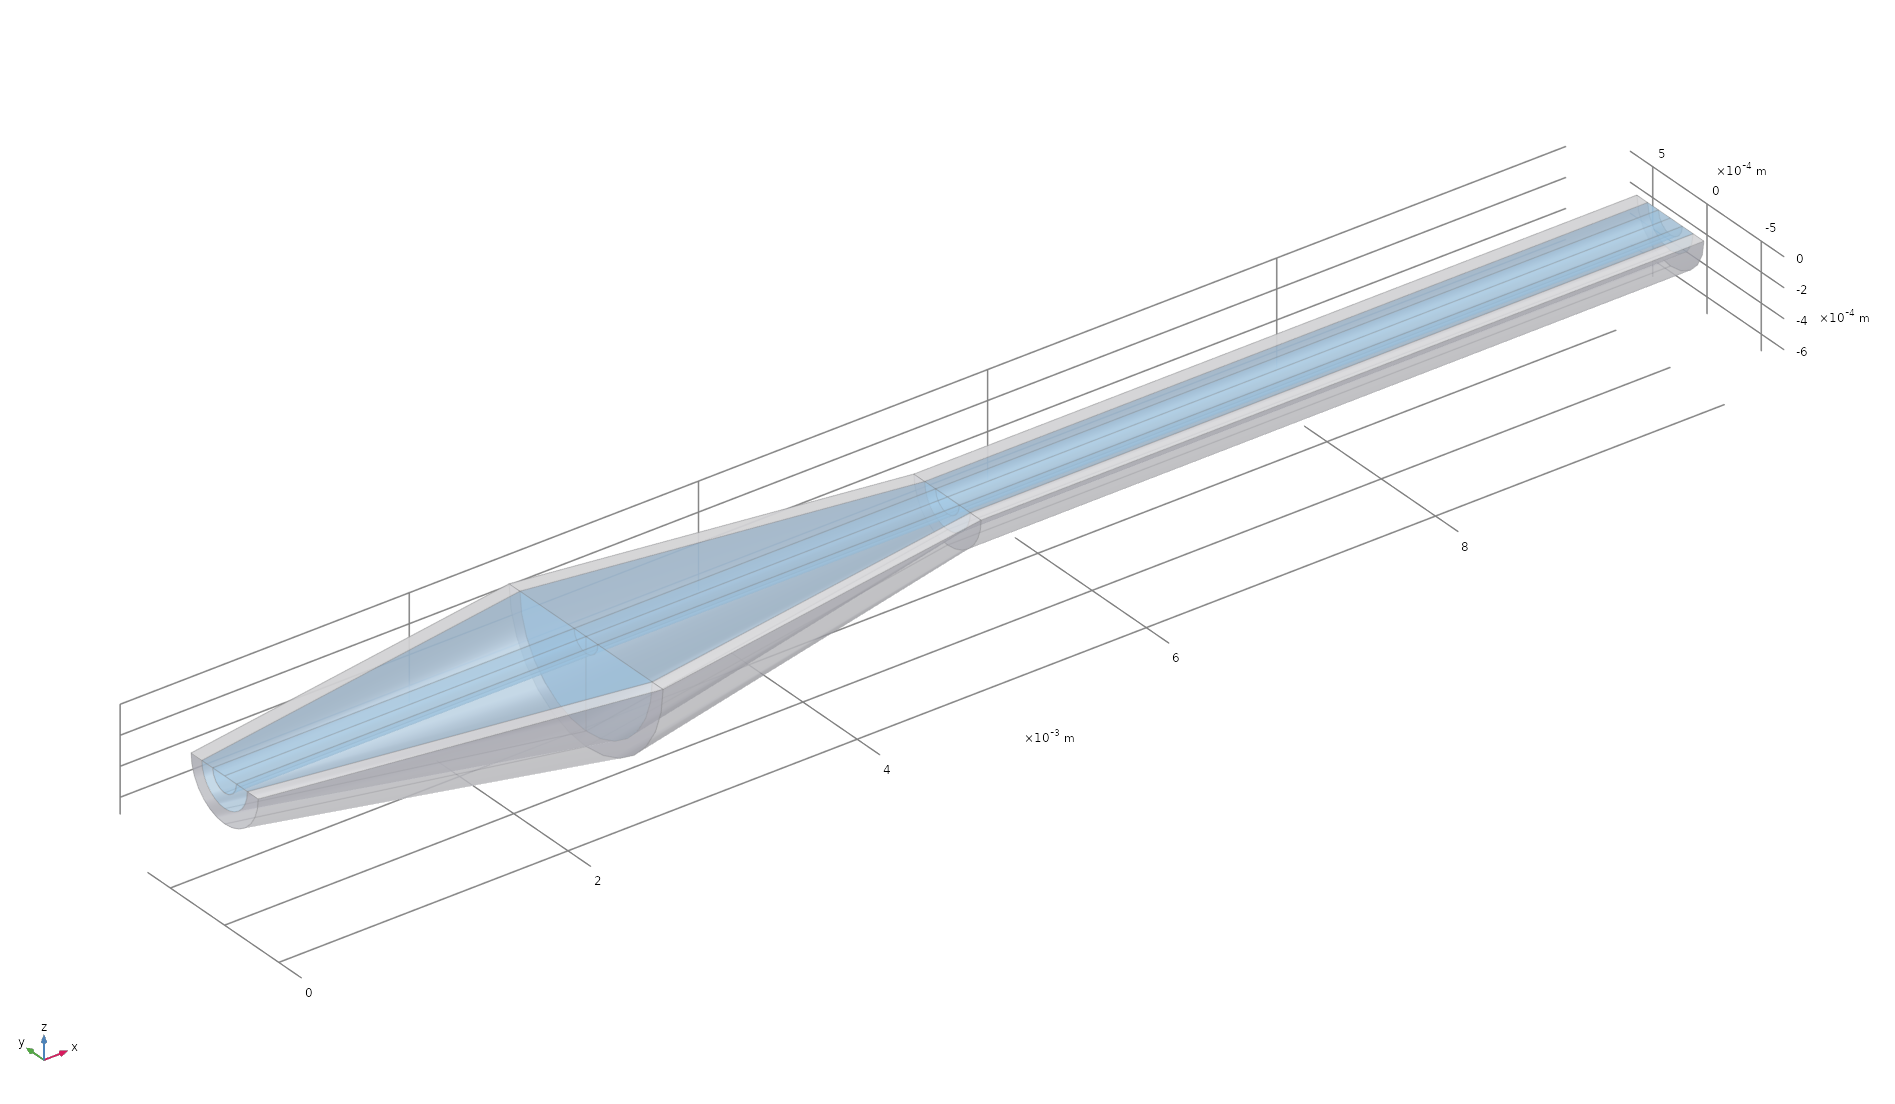
\includegraphics[width = \textwidth]{final_figures/conegeometry.png}
\caption{  {Model geometry wherein ST radius varies longitudinally approximately according to the known anatomy of gerbil, as it appears in the COMSOL Multiphysics user interface. The fluid space (OC, BM and ST) is shown in light blue, while the wall is shown in gray.}}
\label{geometry2}
\end{figure}

\begin{figure}[h]
\centering
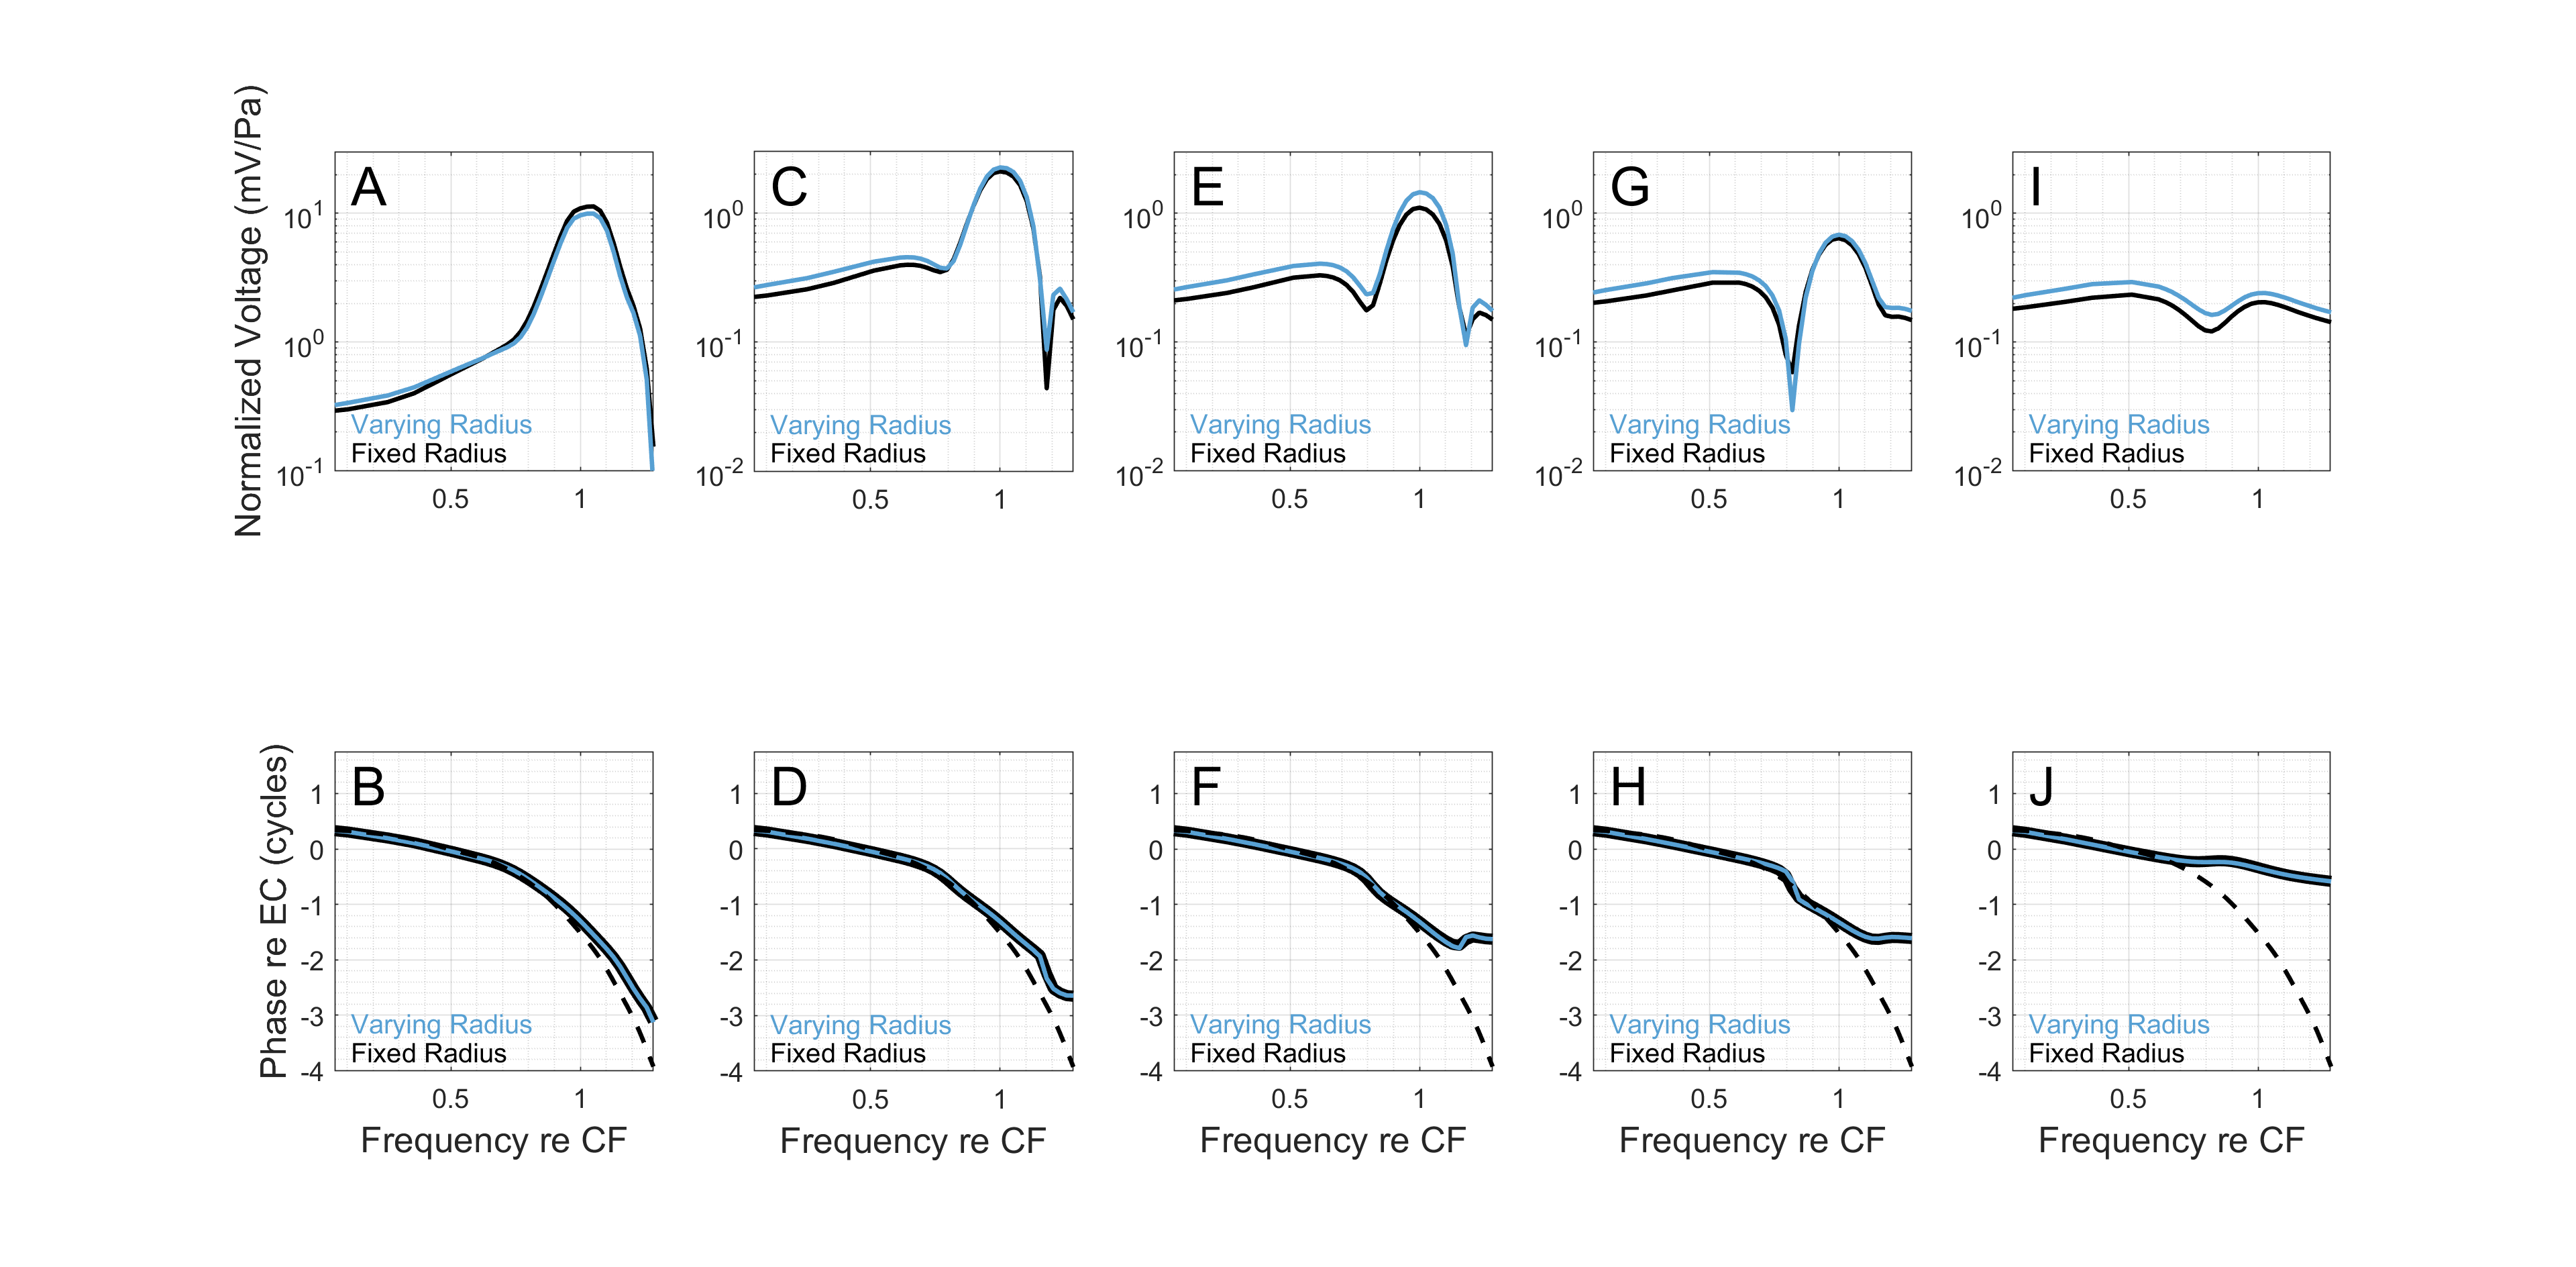
\includegraphics[width = \textwidth]{final_figures/comp geometry.png}
\caption{  {Effect of more accurate geometry.  CM prediction using the current source that is based on BM displacement at five locations along the line segment 2.5 mm from the base of the cochlea (19.5 kHz place), using two model geometries: that from Fig. \ref{geometry2} in which the radius varies, and that from Fig. 1 in the main text  in which the radius is constant. The presented ``fixed radius" results are the predictions from the main text's Fig. 4. SPL = 20 dB SPL, $K=50$, channel sensitivity = 33 pA/nm. Magnitude and phase at the following distances from the current source: \textbf{A} and \textbf{B} -- at the position of the line current source; \textbf{C} and \textbf{D} -- 55 $\mu$m; \textbf{E} and \textbf{F} -- 110 $\mu$m; \textbf{G} and \textbf{H} -- 160 $\mu$m; \textbf{I} and \textbf{J} -- 410 $\mu$m.  The phase of the current source is shown as a dashed line in the lower panels.}}
\label{varyR}
\end{figure}

\begin{figure}[h]
\centering
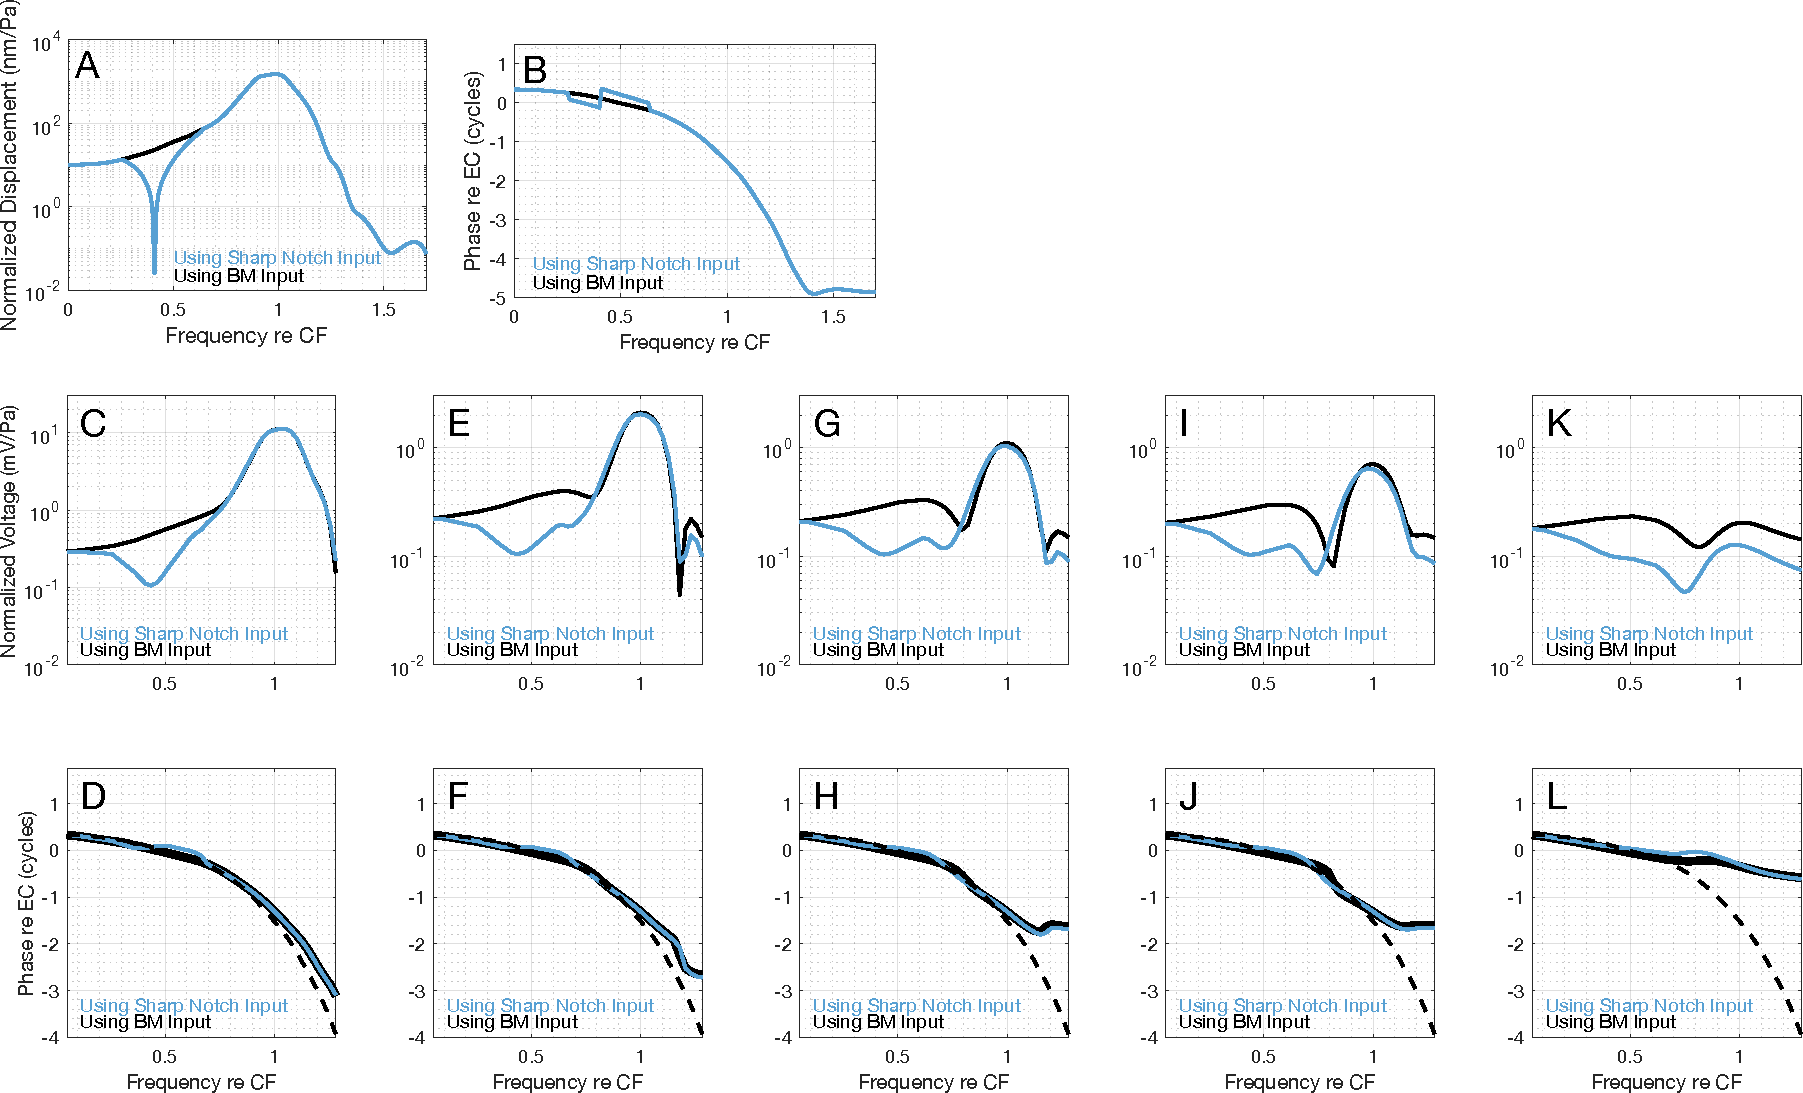
\includegraphics[width = \textwidth]{final_figures/sharpnotchcomp.pdf}
\caption{Effect of a sharp notch in the current source. The notch is added to the original current source based on BM displacement, channel sensitivity = 33 pA/nm, $K=50$,  sound level = 20 dB SPL.  \textbf{A} and \textbf{B} -- magnitude and phase of the inputs with and without the notch.  \textbf{C} through \textbf{L} show CM magnitude and phase at various distances from the current source.  \textbf{C} and \textbf{D} -- at the position of the line-current source; \textbf{E} and \textbf{F} -- 55 $\mu$m; \textbf{G} and \textbf{H} -- 110 $\mu$m; \textbf{I} and \textbf{J} -- 160 $\mu$m; \textbf{K} and \textbf{L} -- 410 $\mu$m. The dashed lines in the lower panels are the phase of the BM displacement used to generate the current stimulus without the notch (as in \textbf{B}).}
\label{notchsharp}
\end{figure}

\begin{figure}[h]
\centering
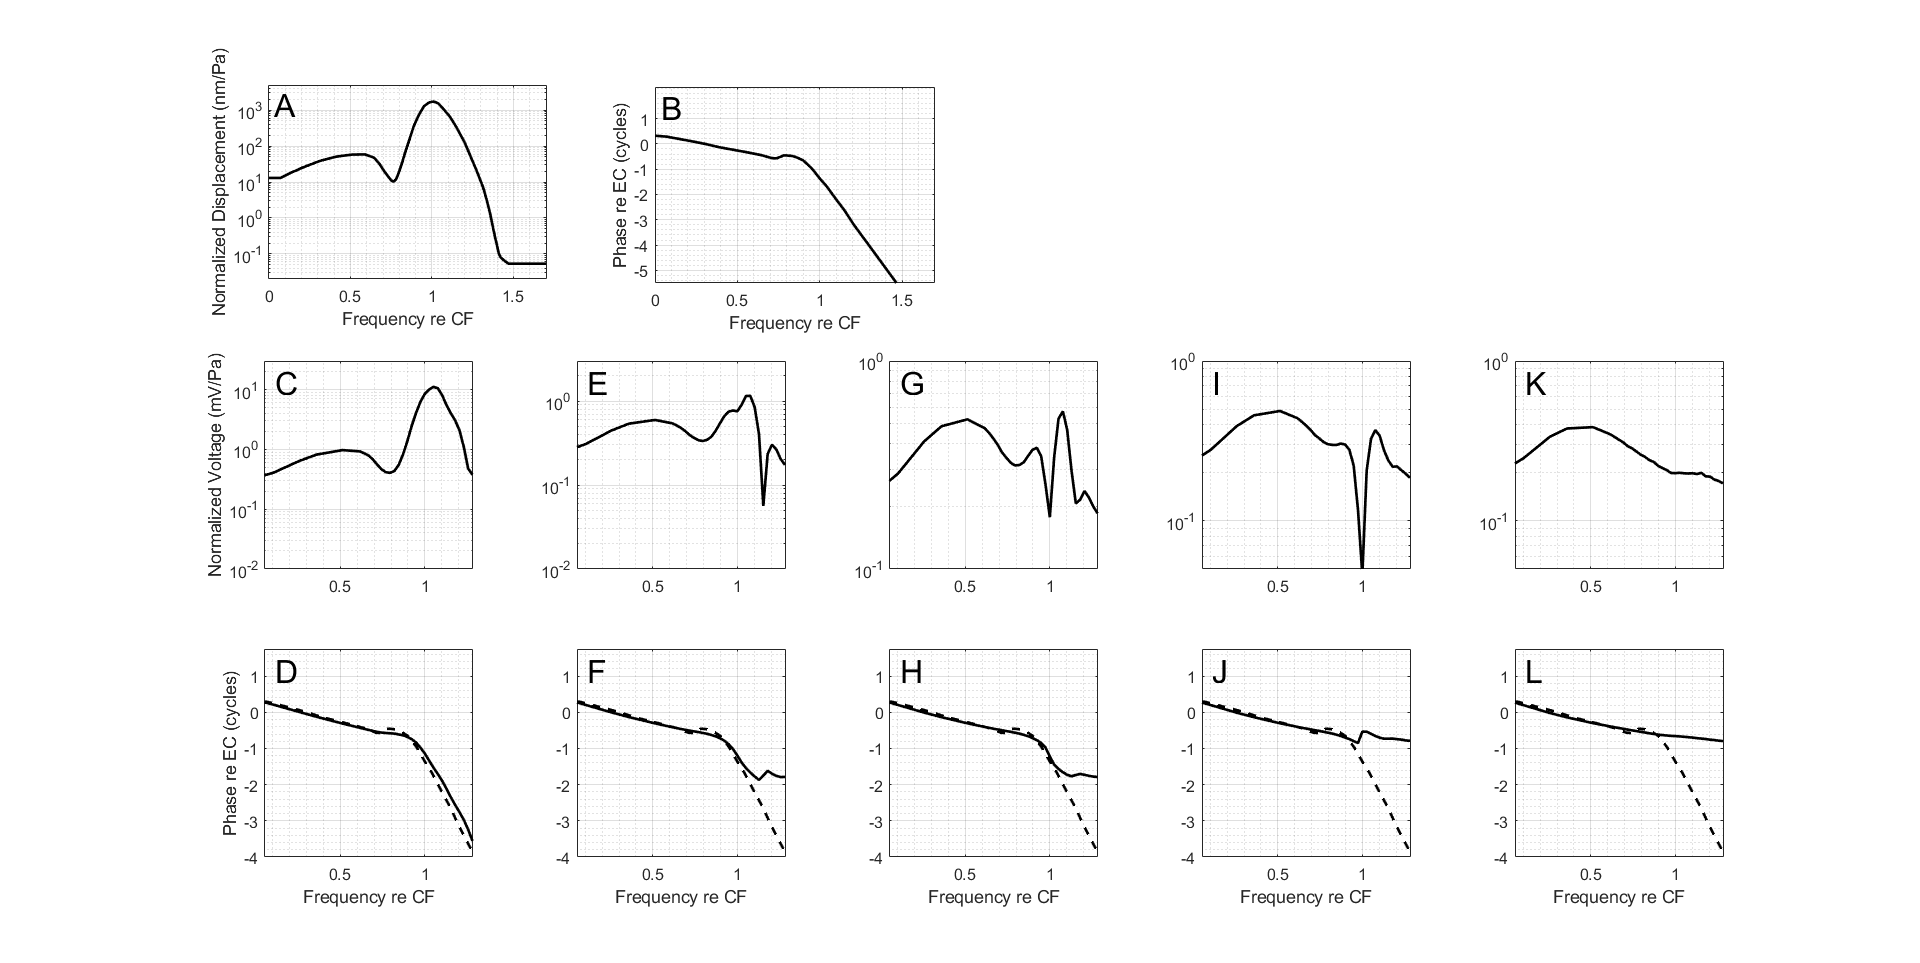
\includegraphics[width = \textwidth]{final_figures/compbroadnotch.png}
\caption{CM prediction where the current source possesses a broad notch and a phase ripple,  inspired by the resonant TM model of Nankali et al, Fig. 5 \cite{nankaliwang}. $K=50$ and channel sensitivity = 33 pA/nm.  \textbf{A} and \textbf{B} -- magnitude and phase of the current source. \textbf{C} through \textbf{L} show CM magnitude and phase at various distances from the current source.  \textbf{C} and \textbf{D} -- at the line-current source; \textbf{E} and \textbf{F} -- 55 $\mu$m; \textbf{G} and \textbf{H} -- 110 $\mu$m; \textbf{I} and \textbf{J} -- 160 $\mu$m; \textbf{K} and \textbf{L} -- 410 $\mu$m. The dashed lines in the lower panels are the phase of the BM displacement used to generate the current stimulus (as in \textbf{B}).}
\label{notchbroad}
\end{figure}


\clearpage

\printbibliography

\end{document}
